%告知 CTeX 这个文件是用 UTF-8 编码
% !Mode:: "TeX:UTF-8"

%使用 pdflatex
%!TEX program = pdflatex


\documentclass[12pt,a4paper]{article}
%正文字体大小为12pt, 页面规格是A4, 使用article文档格式
\usepackage[utf8]{inputenc}
%作用是inputenc用来识别输入编码
\usepackage[left=2.2cm,right=2.2cm,top=3cm,bottom=2.5cm]{geometry}
%latex设置页面边距,页面大小,页边距
\usepackage{mathtools}
%数学公式扩展宏包,提供了公式编号定制和更多的符号、矩阵等
\usepackage{booktabs}  
%booktabs宏包画三线表,线条精细可变
\usepackage{graphicx} 
%支持插图
\usepackage{listings}
%提供了排版关键字高亮的代码环境 lslisting 以及对版式的自定义。
%类似宏包有minted

\lstset{%使用\lstset{}进行代码环境的设置
backgroundcolor=\color{cyan!10},%% 选择代码背景,必须加上\ usepackage {color}或\ usepackage {xcolor}.
basicstyle=\ttfamily, % 设置代码字号.
numbers=left,% 给代码添加行号,可取值none, left, right.
numberstyle=\scriptsize %小六号 \scriptsize
% numberstyle=\tiny\color{mygray}, % 行号的字号和颜色
}

\usepackage{fancyhdr}
%修改页眉页脚格式,令页眉页脚可以左对齐、居中、右对齐

\usepackage{tikz}%以 TikZ 为基础提供排版样式丰富的彩色盒子的功能
\usepackage[europeanresistors,americaninductors]{circuitikz}
%欧式电阻,美式电感

\usepackage{indentfirst} %令章节标题后的第一段首行缩进
\usepackage[wby]{callouts}

\lstdefinestyle{mystyle}{
    backgroundcolor=\color{white},  %背景颜色 
    commentstyle=\color{codegreen}, %注释风格
    keywordstyle=\color{magenta},   %关键字风格 红紫色
    numberstyle=\tiny\color{codegray},
    stringstyle=\color{codepurple},
    basicstyle=\footnotesize\ttfamily,breaklines=true,
    %设置代码的大小  选择一种等宽(“打字机”)字体族  对过长的代码自动换行  
    breakatwhitespace=false, %空格中断
    xleftmargin=20pt, %x左边框
    xrightmargin=20pt,%x右边框       
    breaklines=true,  %代码过长则换行               
    captionpos=b,     % 设置标题位置.               
    keepspaces=true,  % 保留空格    有助于保持代码的缩进 possibly needs columns=flexible           
    numbers=left,     % 给代码添加行号,可取值none, left, right.                   
    numbersep=5pt,    % 设置行号与代码之间的间隔              
    showspaces=false, % 显示每个地方添加特定下划线的空格; 覆盖了'showtringspaces'               
    showstringspaces=false, % 仅在字符串中允许空格
    showtabs=false,   % 在字符串中显示添加特定下划线的制表符               
    tabsize=2,        % 将默认tab设置为2个空格  
    framextopmargin=50pt,%代码区定框
    frame=bottomline,   %代码区底部
    basicstyle=\footnotesize\ttfamily,  % 设置代码字号
    language=Octave     % 使用的语言
}
\usepackage{ulem}%提供排版可断行下划线的命令 \uline 以及其它装饰文字的命令
\lstset{style=mystyle} %代码环境设置  自定义版式,将mystyle中版式导入
\linespread{1.5}       %行距1.5倍 
\title{\textbf{\texttt{Exercises}}}
\author{Automation Class 1904}
\pagestyle{fancy}   %使用fancy风格
\fancyhf{} % 清空当前设置
\rhead{Exercise} %页眉右边
\rfoot{fireowl}       %页脚右边
\lhead{Electric Circuits} % 页眉左边
\cfoot{\thepage}    %页脚中间 页码
\thispagestyle{plain}
% empty
% 无页眉页脚
% plain
% 无页眉,页脚为居中页码
% headings
% 页眉为章节标题,无页脚
% myheadings
% 页眉内容可自定义,无页脚
\date{(Due date: 2020/12/25)}%自定义日期\date{(Due date: 2020/10/5)} \today显示电脑上的日期-英文版


\begin{document}


%section
\begin{enumerate}
	\item
	\begin{quote}
		Find the Thévenin equivalent with respect to the terminals a and b for the circuit in Fig. P4.66.
		\begin{center}
			\begin{circuitikz}[american]
				\draw (0,0) to [V, l=$60V$,-*,invert] (0,3) 
				to [R, l=$10\Omega$] (3,3) 
				to [R, l= $8\Omega$,*-*] (6,3)
				to [short,-*] (8,3);
				\draw (3,3) to[R, l=$40\Omega$, *-*] (3,0);
				\draw(0,0) to[short,-*] (8,0);
				\draw (0,3) to (0,5)
				to [I, l= $6A$] (6,5)
				to (6,3);
				\node at (8,3.2)[blue] {a};
				\node at (8,-0.3)[blue] {b};
			\end{circuitikz}
		\end{center}
	\end{quote}	

    \clearpage
    \item
    \begin{quote}
    	Find the Thévenin equivalent with respect to theterminals a and b for the circuit seen in Fig. P4.77.
    	\begin{center}
    		\begin{circuitikz}[american]
    			\draw (0,0) to [cV, l= $20i_\Delta$, invert] (0,3)
    			to  [R= $10\Omega$, *-*] (3,3) 
    			to [R = $12\Omega$, -*, f_<= $i_\Delta$] (6,3)
    			to [short, -*] (8,3) ;
    			
    			\draw (0,3) to (0,5) to[R = $6\Omega$] (6,5) to (6,3);
    			\draw (3,3) to[R= $2.5\Omega$, -*] (3,0);
    			\draw (0,0) to [short, -*] (8,0);
    			
    			\node at (8,3.3) [blue] {a};
    			\node at (8,-0.3) [blue] {b};
    			
    			\draw (8,0) to [I, l= $1A$]	(8,3);	 
    			
    			\node at(6.3, 2.7) {+};
    			\node at (6.3, 1.5) {$u_T$};
    			\node at (6.3, 0.3) {-};
    			\node at (3, 3.3) [red] {$u_1$};
    			
    		\end{circuitikz}
    	\end{center}
    \end{quote}
   			
    \clearpage
    \item
    \begin{quote}
    	The variable resistor ($R_0$ ) in the circuit in Fig. P4.83 is adjusted until the power dissipated in the resistor is 250 W. Find the values of $R_0$ that satisfy this
    	condition.
    	\begin{center}
    		\begin{circuitikz}[american]
    			\draw (0,0) to [V, l=200V, invert] (0,3) 
    			to [R, l= 25$\Omega$, -*] (3,3)
    			to [R, l = 10$\Omega$, -*] (6,3)
    			to (9,3) to [vR , l= $R_0$] (9,0) to (0,0);
    			
    			\draw (3,3) to [R, l= 100$\Omega$, -*] (3,0);
    			\draw (6,3) to [R, l= $100\Omega$] (6,1.5) to [cV, l= $30i_x$] (6,0);
    			
    			\draw (4,2.6)  [->, -latex, blue] to (5,2.6);
    			\node at (5.3, 2.6) [blue] {$i_x$};
    			
    		\end{circuitikz}
    	\end{center}
    \end{quote}
	
	\clearpage
	\item
	\begin{quote}
		a) In the circuit in Fig. P4.95, before the 10 mA current
		source is attached to the terminals a,b, the
		current $i_0$ is calculated and found to be 3.5 mA.
		Use superposition to find the value of $i_0$ after
		the current source is attached.\\
		b) Verify your solution by finding $i_0$ when all three
		sources are acting simultaneously.
		\begin{center}
			\begin{circuitikz}[american]
				\draw (0,0) to[V, l = 8V, invert] (0,3)
				to (3,3) to [R, l = 2K$\Omega$, *-*] (6,3) to (9,3)
				to [I, l = 10mA, invert] (9,0) to (0,0);
				
				\draw (3,3) to [R, l = 5K$\Omega$, -*] (3,0);
				\draw (6,3) to [R, l = $6K\Omega$, -*] (6,0);
				
				\draw (6,5) to [I, l_= $10mA$] (3,5);
				\draw (3,5) [->, -latex] to (3, 3.1);
				\draw (6,5) [->, -latex] to (6, 3.1);
				
				\node at (2.8, 3.2) {a};
				\node at (6.2, 3.2) {b};
				\node at (5.4, 1.5) [blue]{$i_o$};
				
				\draw (5.6, 2) [->, short, blue] to (5.6,1);
			\end{circuitikz}
		\end{center}
	\end{quote}

	\clearpage
	\item
	\begin{quote}
		Laboratory measurements on a dc voltage source
		yield a terminal voltage of 75 V with no load connected
		to the source and 60 V when loaded with a 20$\Omega$
		resistor.\\
		a) What is the Thévenin equivalent with respect to
		the terminals of the dc voltage source?\\
		b) Show that the Thévenin resistance of the source
		is given by the expression
		\begin{center}
		$R_{Th} = (\frac{v_{Th}}{v_0} - 1)R_L $,
		\end{center}
		where\\
		$v_{Th} = the The´venin voltage,$\\
		$v_0 = the terminal voltage corresponding to the load resistance R_L$
		
		\begin{center}
			\begin{circuitikz}[american]
				\draw (0,0) to [V, l = $V_{Th}$, invert] (0,3)
				to [R, l= $R_{Th}$, -*] (3,3) to (5,3) 
				to [R, l = $30\Omega$] (5,0)
				to [short , -*] (3,0) to (0,0);
				
				\node at (3, 2.7) {+};
				\node at (3,0.3) {-};
				\node at (3, 1.5) {60V};
			\end{circuitikz}
		\end{center}
	\end{quote}
	
	\clearpage
	\item
	\begin{quote}
		The initial voltage on the 0.5$\mu F$ capacitor shown in
		Fig. P6.19(a) is -20V. The capacitor current has
		the waveform shown in Fig. P6.19(b).\\
		a) How much energy, in microjoules, is stored in
		the capacitor at t = 500$\mu F$\\
		b) Repeat (a) for t = $\infty$.
		
		\begin{center}
			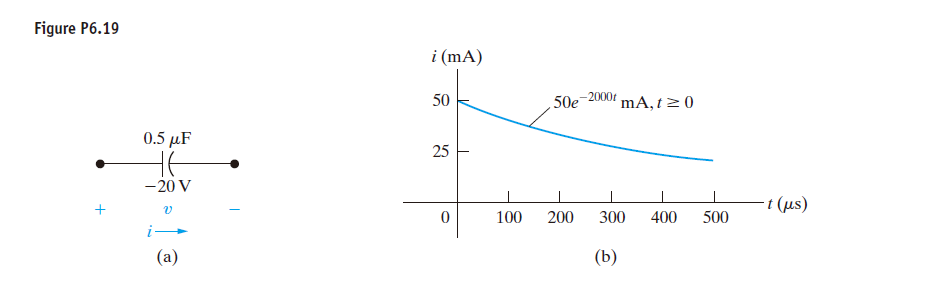
\includegraphics[width=0.75\textheight]{s1_1.png}
		\end{center}
	\end{quote}

	\clearpage
	\item
	\begin{quote}
		The two series-connected capacitors in Fig. P6.31
		are connected to the terminals of a black box at t = 0
		The resulting current i(t) for t $>$ 0 is known
		to be 800$e^{-25t}\mu A$.\\
		a) Replace the original capacitors with an equivalent
		capacitor and find $v_0(t)$ for t $\ge$ 0.\\
		b) Find $v_1(t)$ for t $\ge$ 0.\\
		c) Find $v_2(t)$ for t $\ge$ 0.\\
		d) How much energy is delivered to the black box
		in the time interval 0 $\leq$ t $<$ $\infty$.\\
		e) How much energy was initially stored in the
		series capacitors?\\
		f) How much energyis trapped inthe ideal capacitors?\\
		g) Show that the solutions for $v_1$ and $v_2$ agree with
		the answer obtained in (f).
		
		\begin{center}
			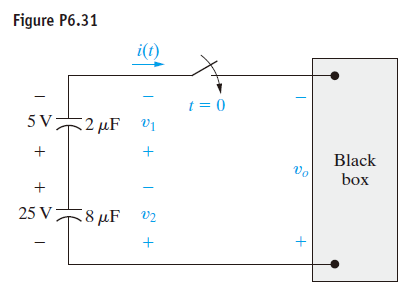
\includegraphics[width= 0.5\textheight]{s1_2.png}
		\end{center}
	\end{quote}
	\clearpage
	Ans7:
	\clearpage
	\item
	\begin{quote}
		The current in the circuit in Fig. P6.35 is known to be
		$i_0 = 3e^{-5000t}(cos2000t + 6sin2000t)A$
		for t$\leq 0^ +.$ Find $v_1(0^+)$ and $v_2(0^+)$.
		
		\begin{center}
			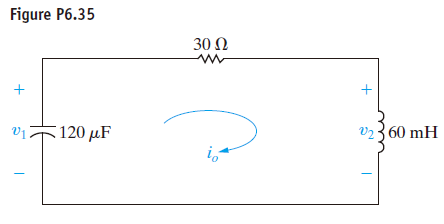
\includegraphics[width= 0.5\textheight]{s1_3.png}
		\end{center}
	\end{quote}





















\end{enumerate}
\end{document}